\section{Implementation, Integration, and Test Plan}
\label{sec:implementation_integration_test}

This section outlines the strategy for the implementation, integration, and testing of the ``Best Bike Paths'' (BBP) system. The process is designed to ensure that the distributed nature of the system (specifically the Thick Client Mobile App and the Fat Server Backend) is robust and scalable.

\subsection{Implementation Plan}
The implementation phase follows an iterative approach, prioritizing the development of core infrastructure components to establish a stable baseline before adding complex features such as automated anomaly detection.

\subsubsection{Development Environment and Tools}
Given the architectural decisions detailed in Section 2, the development environment is structured as follows:

\begin{itemize}
    \item \textbf{Mobile Client (Thick Client - Tier 1):}
    \begin{itemize}
        \item \textbf{Android:} Implemented using Kotlin. Local persistence is managed via \textit{Room} (SQLite abstraction) to support the \textit{Offline-First} pattern.
        \item \textbf{iOS:} Implemented using Swift. Local persistence is managed via \textit{CoreData}.
        \item \textbf{Sensor Logic:} The \textit{Sensor Handler} component requires native implementation to ensure the 50Hz polling frequency required for accurate anomaly detection.
    \end{itemize}
    
    \item \textbf{Backend Server (Fat Server - Tier 2 \& 3):}
    \begin{itemize}
        \item \textbf{Framework:} J2EE Application Server (e.g., Spring Boot) exposing RESTful APIs.
        \item \textbf{Database:} PostgreSQL with the PostGIS extension to handle geospatial data and topology for the \textit{Path Inventory Manager}.
        \item \textbf{Deployment:} Docker containers orchestrated via Kubernetes to support the \textit{Scale-Out} architecture previously described.
    \end{itemize}
\end{itemize}
\clearpage

\subsubsection{Implementation Sequence}
The development is divided into three main milestones:

\begin{enumerate}
    \item \textbf{Milestone 1: Core Infrastructure.} Setup of the Central DBMS and User Account Manager. Implementation of the API Gateway and basic Authentication. Development of the basic Mobile UI and Network Manager.
    
    \item \textbf{Milestone 2: Tracking and Offline Logic.} Implementation of the \textit{Trip Controller} and \textit{Local Storage Manager}. Development of the \textit{Sync Manager} to handle data synchronization and conflict resolution. Integration with External Map Services.
    
    \item \textbf{Milestone 3: Advanced Features.} Implementation of the \textit{Sensor Handler} algorithms for pothole detection. Development of the \textit{Routing Engine} and \textit{Path Inventory Manager} for scoring logic. Integration with External Weather Services for post-trip enrichment.
\end{enumerate}
\clearpage

\subsection{Integration Strategy}
The integration process adopts a \textbf{Continuous Integration (CI)} approach. Given the decoupled nature of the Client and Server (communicating via REST/JSON), integration testing is performed at three levels.

\begin{figure}[h!]
    \centering
    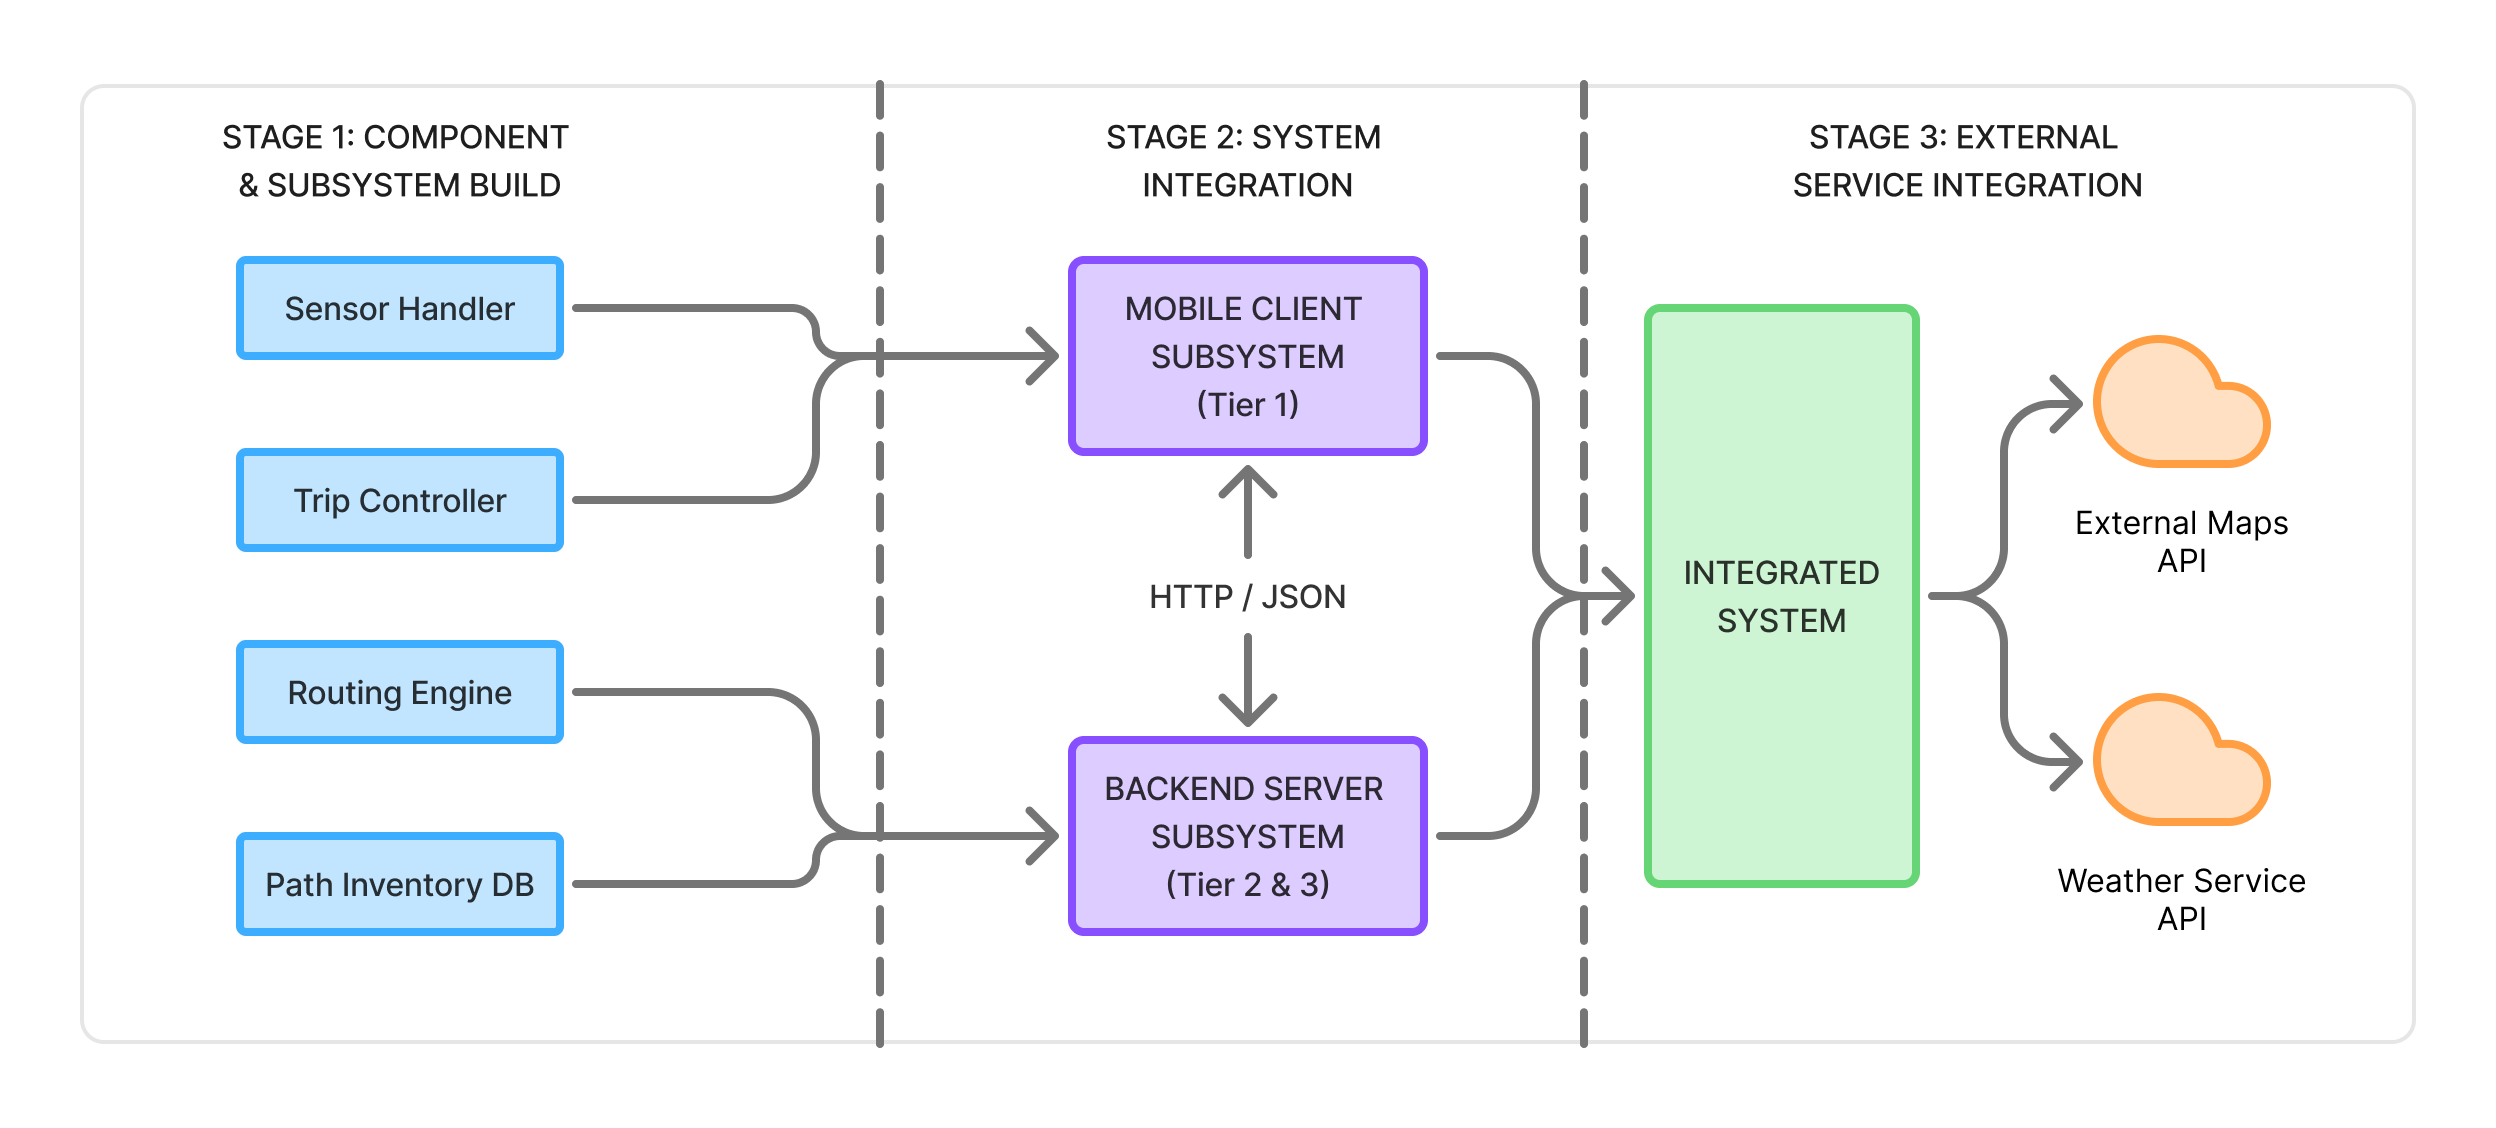
\includegraphics[width=0.9\textwidth]{DD/img/section5/integration.png}
    \caption{Integration Flow Diagram.}
    \label{fig:integration_flow}
\end{figure}

\subsubsection{Subsystem Integration}
\begin{itemize}
    \item \textbf{Client-Side Integration:} The \textit{View Manager}, \textit{Trip Controller}, and \textit{Sensor Handler} are integrated to verify that UI commands correctly trigger background sensor polling. Particular attention is paid to the interaction between the \textit{Sensor Handler} and the \textit{Local Storage Manager} to ensure data is buffered correctly without UI lag.
    \item \textbf{Server-Side Integration:} The \textit{API Gateway} is connected to the internal Managers (\textit{User}, \textit{Trip Processing}, \textit{Inventory}). This step verifies that authenticated requests are correctly routed to the appropriate business logic modules.
\end{itemize}

\subsubsection{System Integration}
This phase connects the Mobile Client to the Backend Server.
\begin{itemize}
    \item \textbf{API Contract Testing:} Verification of JSON request/response structures against the Interface Definitions.
    \item \textbf{Synchronization Testing:} Verifying the \textit{Sync Manager}'s ability to upload batched data and handle network timeouts or server errors.
\end{itemize}

\subsubsection{External Service Integration}
The final integration step involves connecting the Backend Server to third-party providers (Maps and Weather). Mock services are used initially to simulate external API responses during development to avoid rate limits and costs.
\clearpage

\subsection{Test Plan}
The testing strategy is designed to verify both functional requirements and critical non-functional constraints (Performance, Battery, Offline Capabilities).

\begin{figure}[h!]
    \centering
    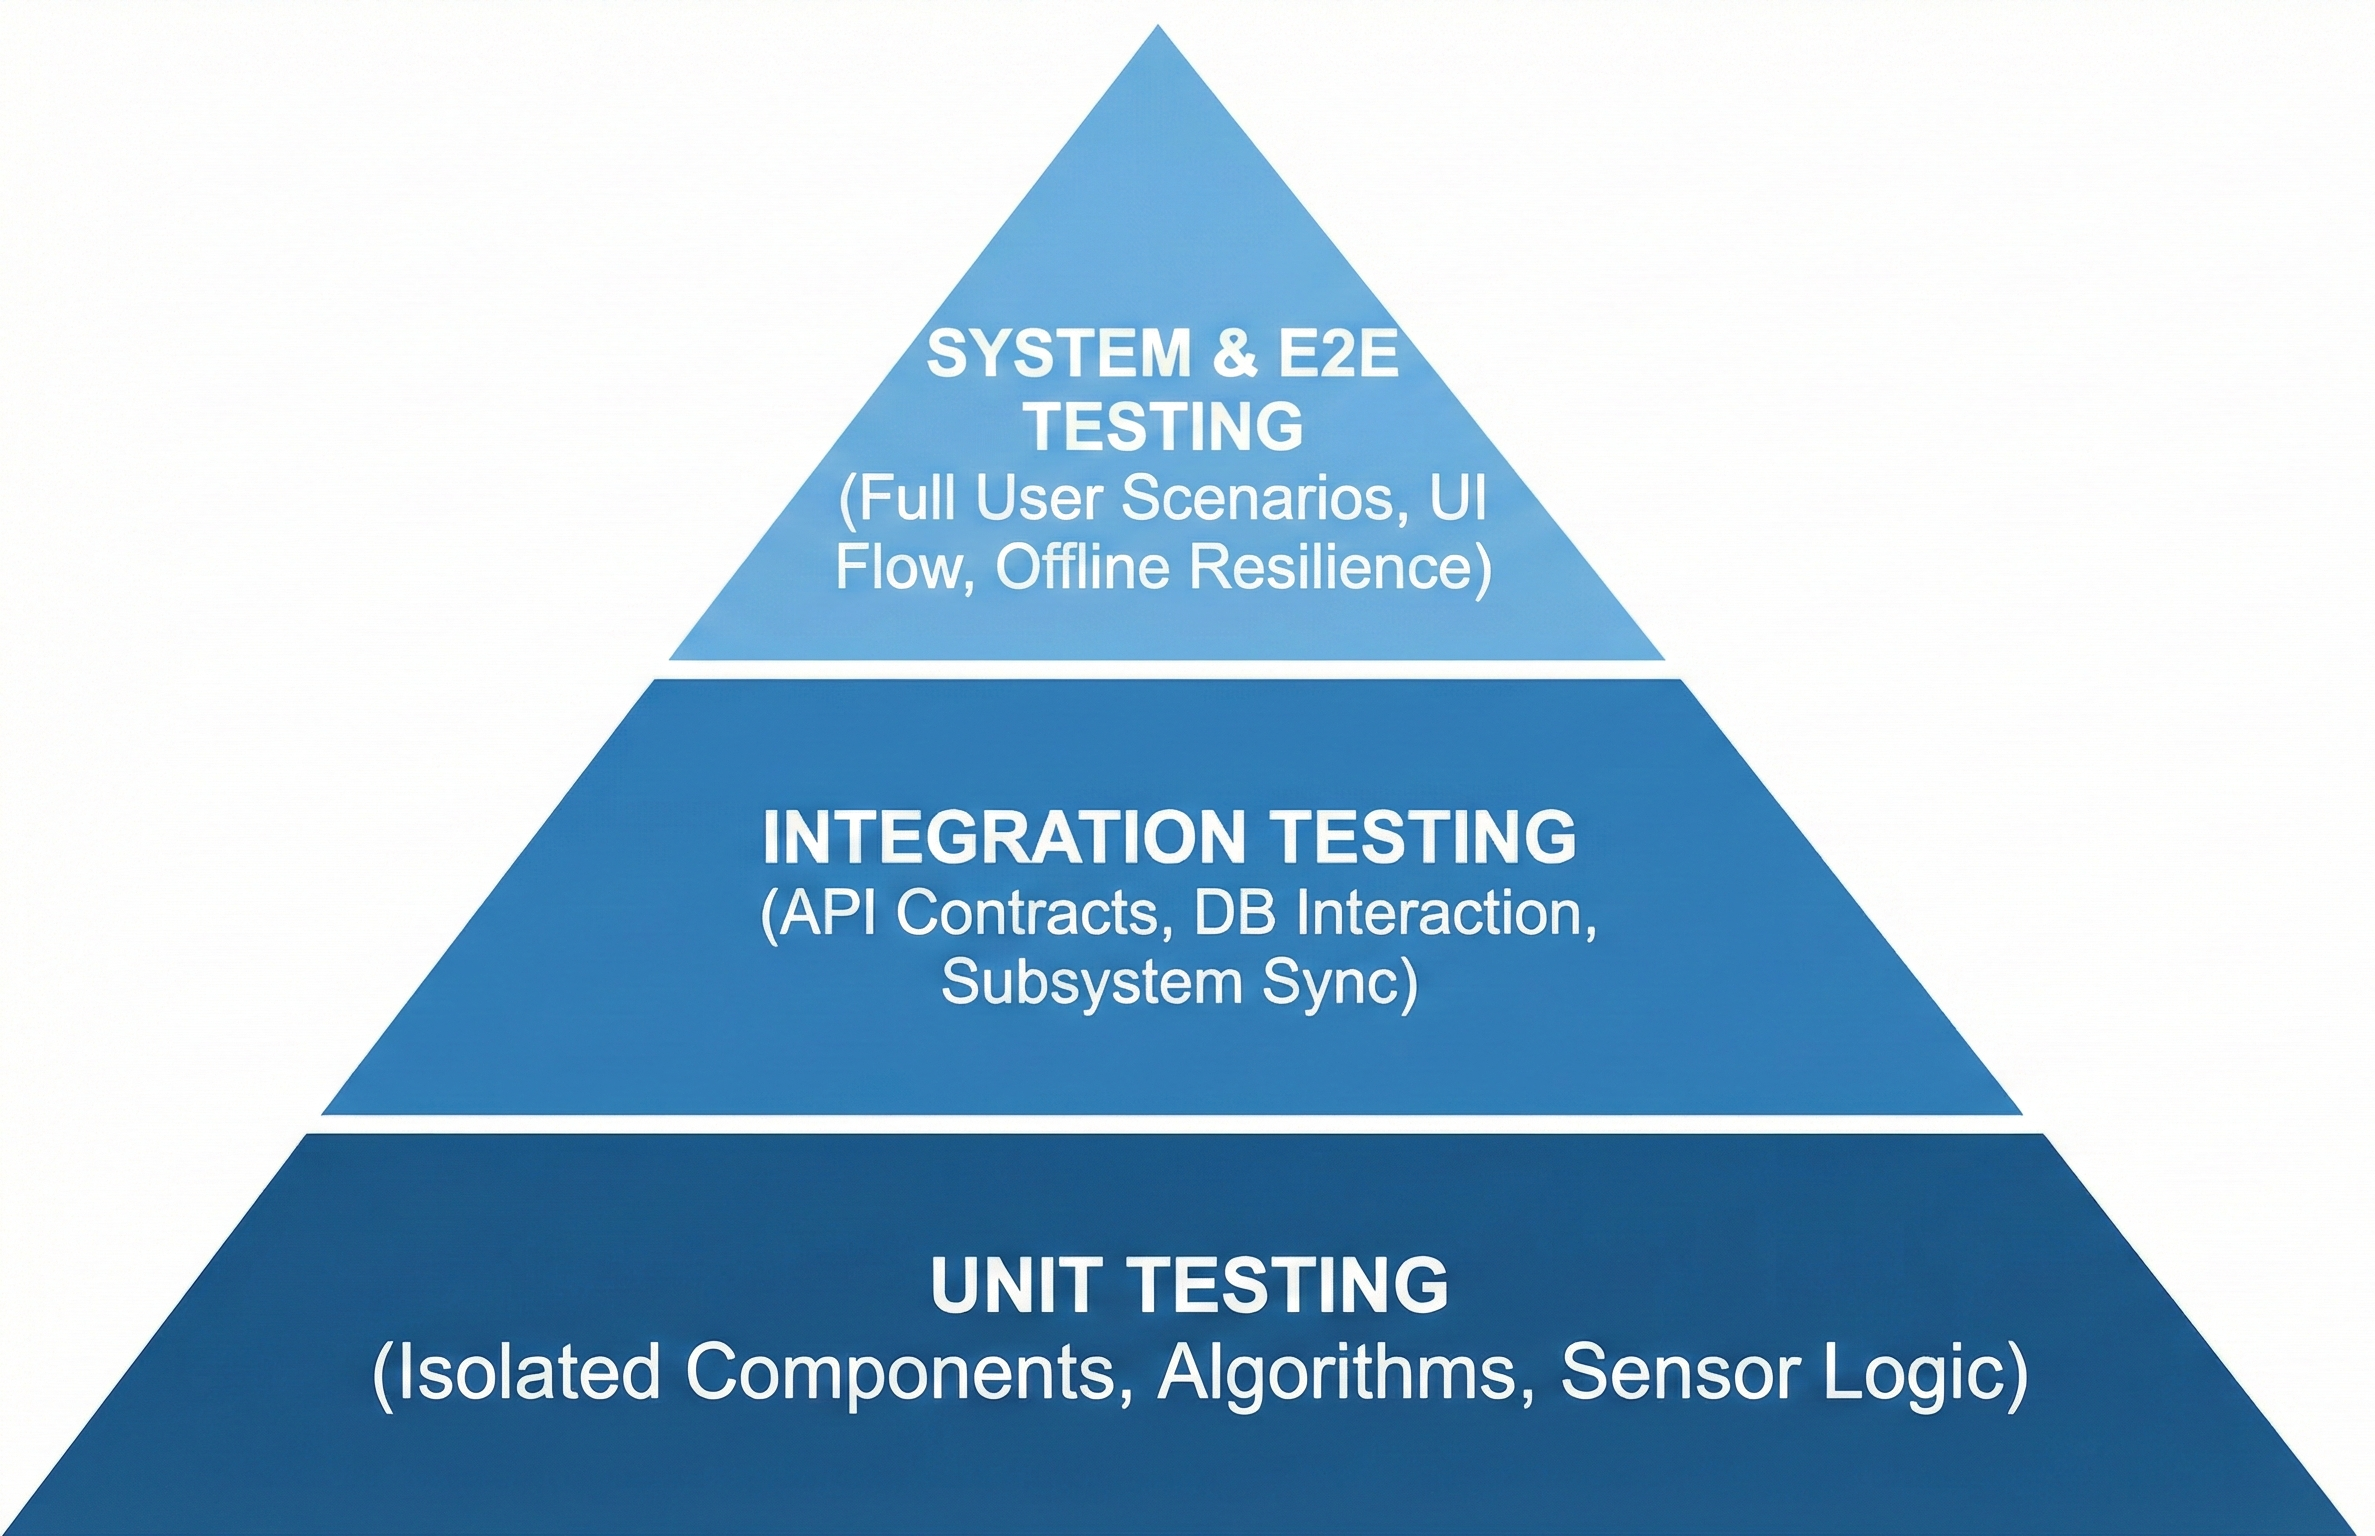
\includegraphics[width=0.7\textwidth]{DD/img/section5/pyramid.png}
    \caption{Testing Strategy Pyramid.}
    \label{fig:testing_pyramid}
\end{figure}

\subsubsection{Unit Testing}
\begin{itemize}
    \item \textbf{Goal:} Verify individual components in isolation.
    \item \textbf{Key Targets:}
    \begin{itemize}
        \item \textbf{Anomaly Detection Algorithm (Client):} Validating that specific accelerometer patterns correctly trigger a ``Suspected Anomaly'' event while filtering out noise.
        \item \textbf{Path Score Calculation (Server):} Verifying that the \textit{Routing Engine} correctly weights distance vs. road quality.
    \end{itemize}
\end{itemize}

\subsubsection{Integration Testing}
\begin{itemize}
    \item \textbf{Goal:} Verify interaction between modules.
    \item \textbf{Key Scenario:} The \textit{Post-Trip Enrichment} flow. Verifying that when a trip is saved, the \textit{Trip Manager} correctly calls the \textit{Weather Connector}, retrieves data, and updates the \textit{Central DBMS} record.
\end{itemize}
\newpage
\subsubsection{System and Acceptance Testing}
This phase involves end-to-end testing of user scenarios defined in the RASD.

\begin{itemize}
    \item \textbf{Offline Resilience Test (Critical):}
    \begin{enumerate}
        \item Start a trip recording.
        \item Physically disconnect the device from the network (Flight Mode).
        \item Continue recording and detecting anomalies.
        \item Stop recording (Verify data is saved locally).
        \item Restore connectivity (Verify \textit{Sync Manager} uploads data automatically).
    \end{enumerate}


    \item \textbf{Battery Consumption Test:}
    \begin{itemize}
        \item Run the application in ``Automated Mode'' for 1 hour on reference devices.
        \item Verify battery drain is within acceptable limits ($< 10\%$).
    \end{itemize}

    \item \textbf{Load Testing (Scalability):}
    \begin{itemize}
        \item Simulate concurrent users sending telemetry updates and requesting routes.
        \item Monitor the \textit{Load Balancer} and Server cluster to ensure response time remains within limits ($< 3$ seconds for route calculation).
    \end{itemize}
\end{itemize}

\subsubsection{Beta Testing}
A closed beta with a selected group of cyclists will be conducted to calibrate the \textit{Sensor Handler} sensitivity in real-world conditions, covering different terrains, bike types, and phone placements.